\item[(a)] Data Generating
Use attached python code to generate the data set.\\
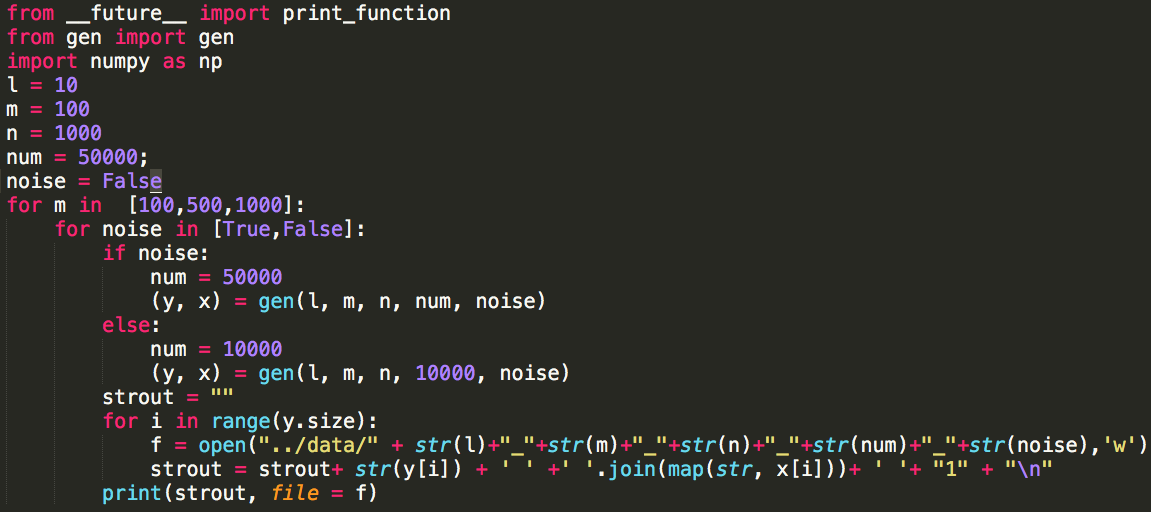
\includegraphics[width = 0.9\textwidth]{pythoncode3.png}

\item[(b)] Parameters Tuning\\
1. For Perceptron, $\eta = 1$, $\gamma = 0$. Nothing needs to be swept.\\ 
2. For Perceptron w/margin, choose $\eta \in \{1.5,0.25,0.03,0.005,0.001\}$, $\gamma = 1$.\\ 
3. For Winnow, choose $\alpha \in \{1.1,1.01,1.005,1.0005,1.0001\}$, $\gamma = 0$.\\
4. For Winnow w/margin, choose $\alpha \in \{1.1,1.01,1.005,1.0005,1.0001\}$, \\$\gamma \in \{2.0,0.3,0.04,0.006,0.001\}$.\\
5. For AdaGrad, choose $\eta \in \{1.5,0.25,0.03,0.005,0.001\}$, $\gamma = 1$.\\
Input 10\% of noisy data as training data and another 10\% of data as testing data.
\end{itemize}
   \begin{center}
    \begin{tabular}{|p{2.2cm}|p{1.2cm}|p{2cm}|p{1.2cm}|p{2cm}|p{1.2cm}|p{2cm}|}
      \hline
      Algorithm &\multicolumn{2}{|c|}{m=100}& \multicolumn{2}{|c|}{m=500} & \multicolumn{2}{|c|}{m=100}\\\hline\hline
       &  Accu. &   params.  &  Accu. &   params. &  Accu. &   params.\\\hline
      Perceptron &  0.8012 &  NA &  0.5456&  NA&  0.688& NA \\\hline
      Perceptron w/margin & 0.8232 &  $\eta$=0.005 &  0.6534&  $\eta$=0.03 &  0.7174&$\eta$=0.03 \\\hline
      Winnow   & 0.8778 &  $\alpha$=1.1 &  0.7934&  $\alpha$=1.1&  0.7356&$\alpha$=1.1\\\hline
      Winnow w/margin&   0.8778 &  $\alpha$=1.1, $\gamma$=0.006 &  0.7994&  $\alpha$=1.1, $\gamma$=0.04&  0.7424 & $\alpha$=1.1, $\gamma$=0.04 \\\hline
      AdaGrad  & 0.8766 &  $\eta$=0.25 &  0.7788&  $\eta$=1.5&  0.7352&$\eta$=1.5\\\hline
    \end{tabular}
\end{center}
\clearpage
\begin{itemize} 
  \item[(c)] Experiment\\
  Use the parameters acquired before and input 50000 training noisy examples and test it with 10000 clean test examples. 
\begin{center}
    \begin{tabular}{|p{2.2cm}|p{1.2cm}|p{2cm}|p{1.2cm}|p{2cm}|p{1.2cm}|p{2cm}|}
      \hline
      Algorithm &\multicolumn{2}{|c|}{m=100}& \multicolumn{2}{|c|}{m=500} & \multicolumn{2}{|c|}{m=1000}\\\hline\hline
       &  Accu. &   params.  &  Accu. &   params. &  Accu. &   params.\\\hline
      Perceptron &  0.973 &  NA &  0.8114&  NA&  0.7709& NA \\\hline
      Perceptron w/margin & 0.9924 &  $\eta$=0.005 &  0.9084&  $\eta$=0.03 &  0.8308&$\eta$=0.03 \\\hline
      Winnow   & 0.9663 &  $\alpha$=1.1 &  0.9366&  $\alpha$=1.1&  0.7708&$\alpha$=1.1\\\hline
      Winnow w/margin&   0.9536 &  $\alpha$=1.1, $\gamma$=0.006 &  0.9245&  $\alpha$=1.1, $\gamma$=0.04&  0.7699 & $\alpha$=1.1, $\gamma$=0.04 \\\hline
      AdaGrad  & 0.9998 &  $\eta$=0.25 &  0.991&  $\eta$=1.5&  0.8591&$\eta$=1.5\\\hline
    \end{tabular}
\end{center} 
According to the table above, the sparser dataset is the better AdaGrad is comparing to others. Winnow thought to be the best in the past 2 experiments does a bad job in the sparse data. 